\documentclass{article}

\usepackage[a4paper, total={18.2cm, 27cm}]{geometry}
\usepackage{txfonts}
\usepackage{graphicx}
\usepackage[spanish, es-nodecimaldot]{babel}
\usepackage{float}
\usepackage[figurename=Figura]{caption}
\usepackage[numbers, sort&compress]{natbib}
\usepackage[hyphens]{url}
\usepackage{indentfirst}
\usepackage{hyperref}
\usepackage{xcolor}


\date{\textbf{Candidato: Diego Antonio Román Cortés\\ Profesor Guía: Rodrigo Andrés Vicencio Poblete}}
\author{Proyecto de Tesis para optar al grado de Magíster en Ciencias, mención en Física}
\title{Redes multiorbitales basadas en moléculas fotónicas}

\begin{document} \maketitle
%Título del proyecto
%Nombre del candidato y del profesor guía o profesores guía

\section{Contexto del proyecto}

Entre los premios Nobel en Física de la última década \cite{nobel} se encuentran varios que están estrechamente ligados a la óptica: por la generación de pulsos de luz ultra cortos (femtosegundos \cite{femto1} y luego attosegundos \cite{atto1, atto2, atto3}), por experimentos con fotones entrelazados \cite{photons1, photons2, photons3}, por la ideación de pinzas ópticas \cite{opticaltweezers} y por la invención de luces LED \cite{led1, led2, led3}. El estudio del comportamiento de la luz en diversos contextos ha permitido el posterior desarrollo tecnológico con aplicaciones industriales, en medicina, en comunicaciones e incluso militares. Una aplicación cotidiana es la fibra óptica, que actúa como una guía de onda para la luz y actualmente es el principal medio de transmisión de Internet en el mundo \cite{fibra2, fibra}. 
	
	Numerosos de estos avances en el control de las propiedades de transporte de la luz se han visto propiciados por la técnica de escritura de guías de onda por láser de femtosegundos, la cual ha permitido la fabricación de redes fotónicas de variada índole \cite{femto, bics, lieb1, lieb2, artificialFB, FBdynamics, strain, dendritas, splitters}. Su importancia radica no sólo en emular situaciones de la física del sólido, tales como oscilaciones de Bloch \cite{BlochOsci}, localización de Anderson \cite{Anderson}, estados de banda plana \cite{lieb1, lieb2, artificialFB, FBdynamics} o topología \cite{obstopo, obsfloquet, topo1dphoto,toporusos}, sino que también en el estudio de fenómenos ópticos incluyendo no-linealidad tipo Kerr y su uso en la formación de solitones \cite{discretesolitons}, la posible propagación de luz cuántica \cite{qed, squeezed, topoquantum}, o su compatibilidad con la transmisión de información en la industria de las telecomunicaciones \cite{telecom}.
	
	El enfoque de este proyecto será el estudio de redes fotónicas multiorbitales. Por ello será crucial incorporar la técnica de acoplamiento interorbital, que consiste en sintonizar las constantes de propagación de el modo fundamental de una guía monomodal (S) con el primer modo guiado excitado de una guía dimodal (P) mediante la calibración adecuada de las potencias de escritura, que inducen diferencias en los contrastes generados por la técnica de escritura por láser femtosegundos \cite{interorbital}.
	
	El llamado acoplamiento SP ha permitido el estudio de redes que presentan flujo magnético efectivo $\Phi = \pi$, el cual permite el transporte controlado de la luz \cite{OAMCaging, ABCaging}. Una aplicación directa de este fenómeno es la generación de guías de onda que admitan modos guiados de luz con momentum angular orbital (OAM) y la codificación de su carga topológica $\ell$ como medio para transmitir información \cite{oamapp, oamfree}. Se ha reportado a la fecha sólo la propagación de OAM mediante de redes fotónicas que presevan simetría $C_3$ \cite{OAMWG, vortex}. Sin embargo, el acoplamiento entre modos OAM en una red fotónica permitiría la generación de flujos magnéticos distintos de $0$ o $\pi$, lo que se reflejaría en una direccionalidad dependiente de la circulación propagante \cite{vortextrim, topoOAM}. Para ello será necesario introducir el concepto de ``moléculas fotónicas'' \cite{molecules} y estudiar su aplicación en redes fotónicas \cite{SPSSH}.
\section{Objetivos de la tesis}
\begin{enumerate}
	\item Explorar la utilización de moléculas fotónicas como base para fabricar y estudiar redes interorbitales.
	\item Entender el comportamiento de los modos guiados en moléculas fotónicas y su interacción en el régimen de acoplamiento débil.
\end{enumerate}
\section{Metodología}

Desde las ecuaciones de Maxwell en un medio dieléctrico no magnético sin cargas ni corrientes libres es posible escribir la siguiente ecuación para la envolvente lenta del campo eléctrico $\textbf{E}(\textbf{r}) = \textbf{E}_1(\textbf{r}) e^{-i \textbf{k}_1 \cdot \textbf{r}}$,

\begin{equation}
	(\nabla-i\textbf{k}_1)\times((\nabla-i\textbf{k}_1)\times \textbf{E}_1) = k^2 \textbf{E}_1,
	 \label{eqn:maxwell}
\end{equation}
con $k \equiv k_0 n(x,y,z)$.
La ecuación (\ref{eqn:maxwell}) se puede resolver vía el software comercial COMSOL \textit{Multiphysics} mediante elementos finitos, y que será una de las herramientas de esta tesis. Por otro lado, utilizando la aproximación paraxial escogiendo el eje $z$  como dirección de propagación y seleccionando la polarización horizontal del campo, es posible simplificar la ecuación (\ref{eqn:maxwell}) y llegar a la formulación de un método numérico escalar conocido como \textit{Beam Propagation Method}, utilizado ampliamente en esta área de investigación \cite{bics, interorbital, OAMCaging, vortex, bpm}. Éste consiste en resolver numéricamente la ecuación
\begin{equation}
	2in_0k_0\frac{\partial}{\partial z}\psi(x,y,z) = \nabla_\perp^2 \psi (x,y,z) + \left(n^2-n_0^2\right)k_0^2 \psi (x,y,z), \label{eqn:paraxial}
\end{equation}
con $\psi(x,y,z)$, $n_0$ , $n(x,y)$ y $k_0$ la envolvente de la componente horizontal campo eléctrico, el índice de refracción del material, el índice de refracción inducido y el número de onda en el vacío, respectivamente. Aplicando teoría acoplada de modos \cite{coupledmodetheory} a la ecuación (\ref{eqn:paraxial}), con el objetivo de describir de forma discreta una red fotónica, es posible derivar las llamadas ecuaciones discretas tipo Schrödinger \cite{discretesolitons, artificialFB, FBdynamics}
\begin{equation}
	-i\frac{\partial u_{\vec{n}} }{\partial z} = \beta_{\vec{n}}u_{\vec{n}} + \sum_{\vec{m}\neq\vec{n}} C_{\vec{n},\vec{m}}u_{\vec{m}}, \label{eqn:CMT}
\end{equation}
con $u_{\vec{n}}, \beta_{\vec{n}}$ y $C_{\vec{n}, \vec{m}}$ la envolvente normalizada del campo eléctrico, la constante de propagación normalizada y las constantes de acoplamiento entre los modos de las guías en las posiciones de la red $\vec{n}$ y $\vec{m}$, respectivamente.


Para la fabricación de guías de onda se utiliza un láser femtosegundo pulsado de 1030 nm enfocado en un vidrio de borosilicato en movimiento gracias a una plataforma XYZ motorizada, como se ilustra en la Figura \ref{fig:femtosetup} a): 

\begin{figure}[H]
	\centering
	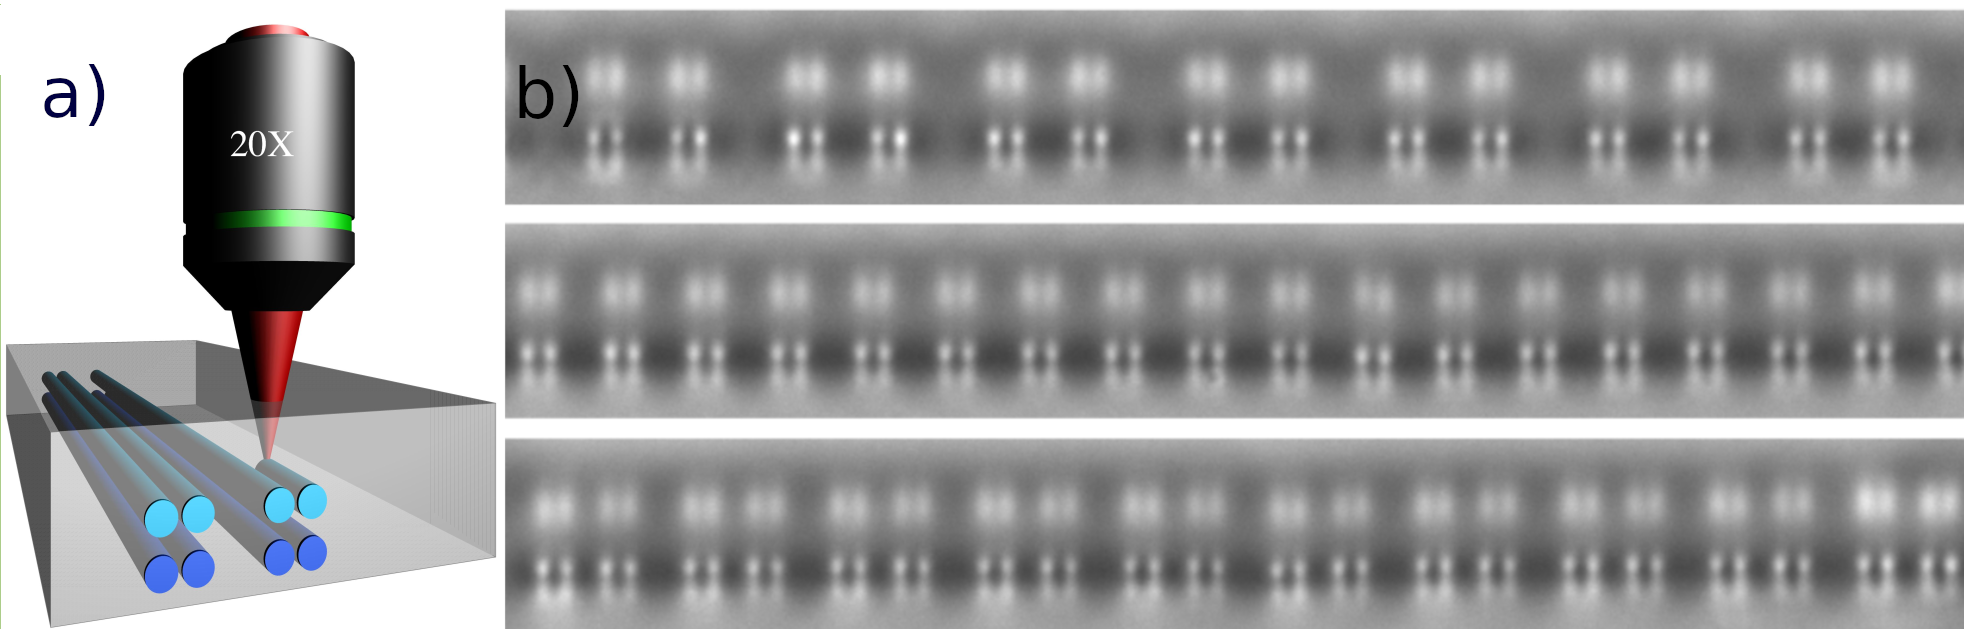
\includegraphics[width=0.7\linewidth]{./media/femtosetup.png}
	\caption{a) Montaje de fabricación de guías de onda mediante el enfoque de un láser de femtosegundo. b) Imagen microscópica de la cara salida iluminada con luz blanca de una red multiorbital con moléculas fotónicas. \label{fig:femtosetup}}
\end{figure}


La excitación de redes fotónicas interorbitales hace necesario el uso de condiciones iniciales no triviales. Para ello el estudiante implementó, como trabajo previo, una técnica de modulación espacial de luz que permite modular tanto la amplitud como la fase de la luz proveniente de un láser de 730nm, cuyo esquema simplificado se ilustra en la Figura \ref{fig:SLM}. Esto se logra mediante un $\lambda/2$ para que la polarización coincida con la respuesta del Cristal Líquido (PLUTO-NIR: SLM - Reflective LCOS). Se utiliza un lente objetivo 20x seguido de un lente de 150 mm para ensanchar y colimar el haz. El primer \textit{Beam Splitter} (BS) permite tener una referencia para realizar interferometría a la salida del monetaje. La modulación es controlada por el software HOLOEYE que recibe imágenes en blanco y negro que codifican la intensidad de voltaje aplicado en cada píxel del modulador. Como un PLUTO-NIR sólo es capaz de modular la fase, se utiliza primero un holograma de gradiente de fase (\textit{blaze grating}) al que se le aplica una máscara de intensidad y finalmente se agrega la fase deseada, técnica conocida \textit{Phase Imprinting Technique} \cite{slm}. Para acoplar la modulación con los modos micrométricos de las guías de onda, es necesario usar dos lentes de 1000 mm y 50 mm que reduzcan el tamaño de la imagen. Dos lentes objetivos 4x se usan luego de un BS una vez puesta la muestra para calibrar los planos de imagen de 1) la cara de entrada de la muestra (iluminada con luz blanca) con 2) el holograma que se refleja desde la cara de entrada usando una cámara CCD. Finalmente, la luz propagada en la muestra es capturada por un lente objetivo 10x y enfocada en otra cámara CCD tipo \textit{Beam Profiler}. Opcionalmente, se puede colocar otro BS para obtener información sobre la fase de la imagen mediante técnicas de interferometría.

\begin{figure}[H]
	\centering
	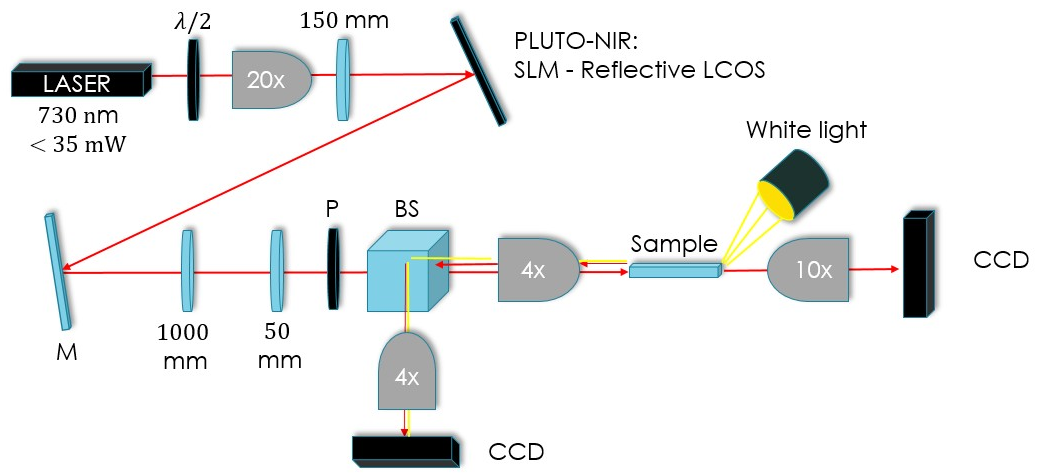
\includegraphics[width=0.7\linewidth]{./media/SLMsetup.png}
	\caption{Montaje de excitación de guías de onda con condiciones iniciales moduladas en amplitud y fase.\label{fig:SLM}}
\end{figure}



Para ciertos experimentos resulta más apropiada la excitación de redes fotónicas variando la longitud de onda de excitación \cite{spectraltransfer, SPSSH}. Para ello se utiliza el montaje ilustrado en la Figura \ref{fig:supercontinuum}, el que está basado en un láser supercontinuo con un espectro de 400-2000 nm:

\begin{figure}[H]
	\centering
	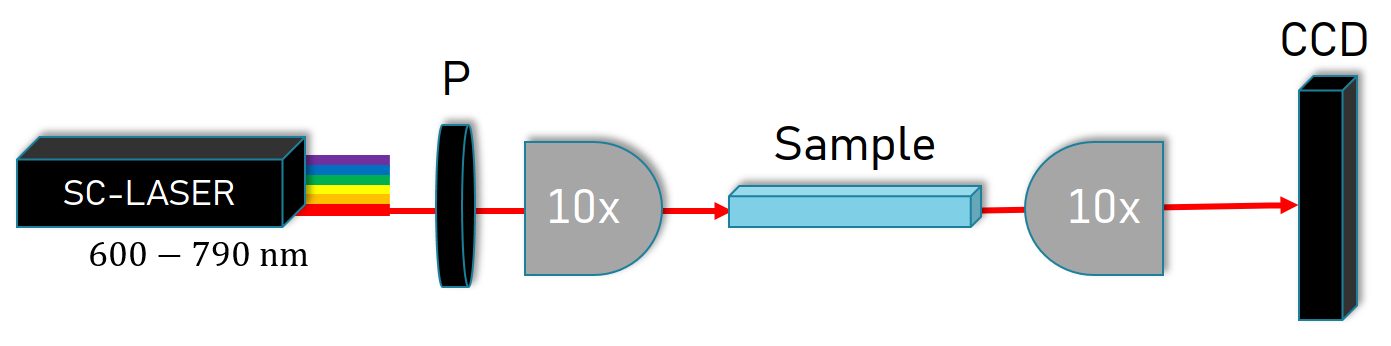
\includegraphics[width=0.5\linewidth]{./media/supercontinuum.png}
	\caption{Montaje de excitación de guías de onda con distintas longitudes de onda.\label{fig:supercontinuum}}
\end{figure}


\section{Trabajo adelantado}

Se hizo un barrido de parámetros de fabricación de guías de onda, en particular de potencia de escritura y separación entre guías, logrando la inversión de elipticidad, el sintonizado de las constantes de propagación del modo fundamental $S$ de la molécula de excitación y el modo excitado $P_x$ de la molécula de acoplamiento, optimizado para 730 nm.


\begin{figure}[H]
	\centering
	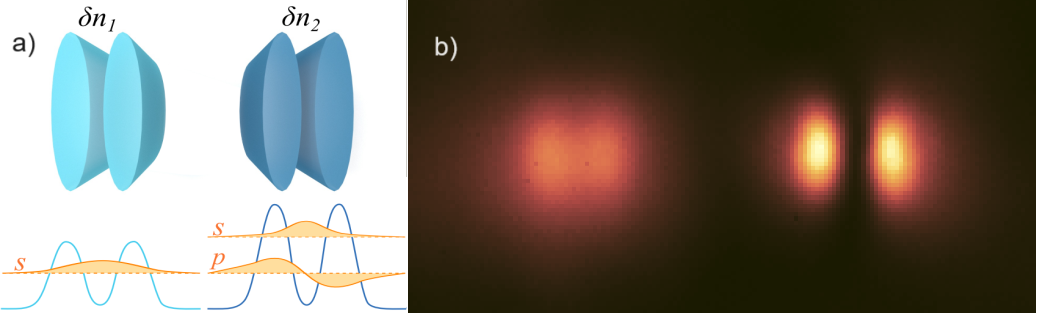
\includegraphics[width=0.7\linewidth]{./media/detuningv2.png}
	\caption{a) Ilustración del concepto de moléculas fotóncias y del sintonizado de las constantes de propagación modificando los índices de refracción. b) Interacción interorbital en moléculas fotónicas a 25 $\mu$m de separación y 13 mm de propagación. Se inyecta luz láser en la molécula S ubicada a la izquierda.}
\end{figure}

Esta sintonización permitió la fabricación de las redes SP-SSH mostradas en la Figura \ref{fig:femtosetup}b) y estudiadas tanto teórica, numérica y analíticamente en las referencias \cite{toporusos, topo1dphoto, SPSSH}.

Con parámetros de fabricación similares se fabricaron redes 1D-SP, las cuales exhiben una transición entre localización y transporte en función de la longitud de onda de excitación. La excitación experimental mediante láser supercontinuo se presenta en la figura \ref{fig:super} en 50 mm de propagación.

\begin{figure}[H]
	\centering
	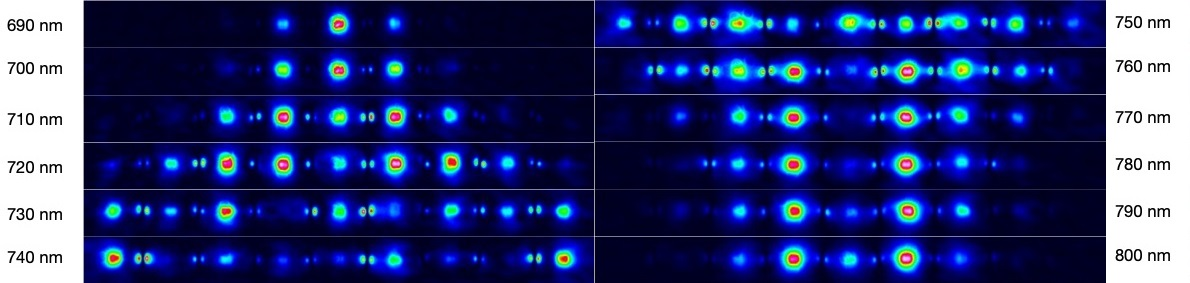
\includegraphics[width=1.0\linewidth]{./media/SP1D.jpg}
	\caption{Excitación de bulto de la red 1D SP variando la longitud de onda de excitación. \label{fig:super}}
\end{figure}

Luego de implementar el montaje de modulación esquematizado en la Figura \ref{fig:SLM}, fue posible la excitación precisa de un dipolo horizontal. Con ello se hizo un estudio del comportamiento del acoplamiento de modos P al variar el ángulo entre moléculas P. En la Figura \ref{fig:dipoles}d) el acoplamiento dipolar se acerca a cero, lo que se asemeja al valor de ángulo $\theta$ que hace nulo el término de interacción dipolar $\cos^2(\theta_{magic}) = \frac{1}{3}$.  

\begin{figure}[H]
	\centering
	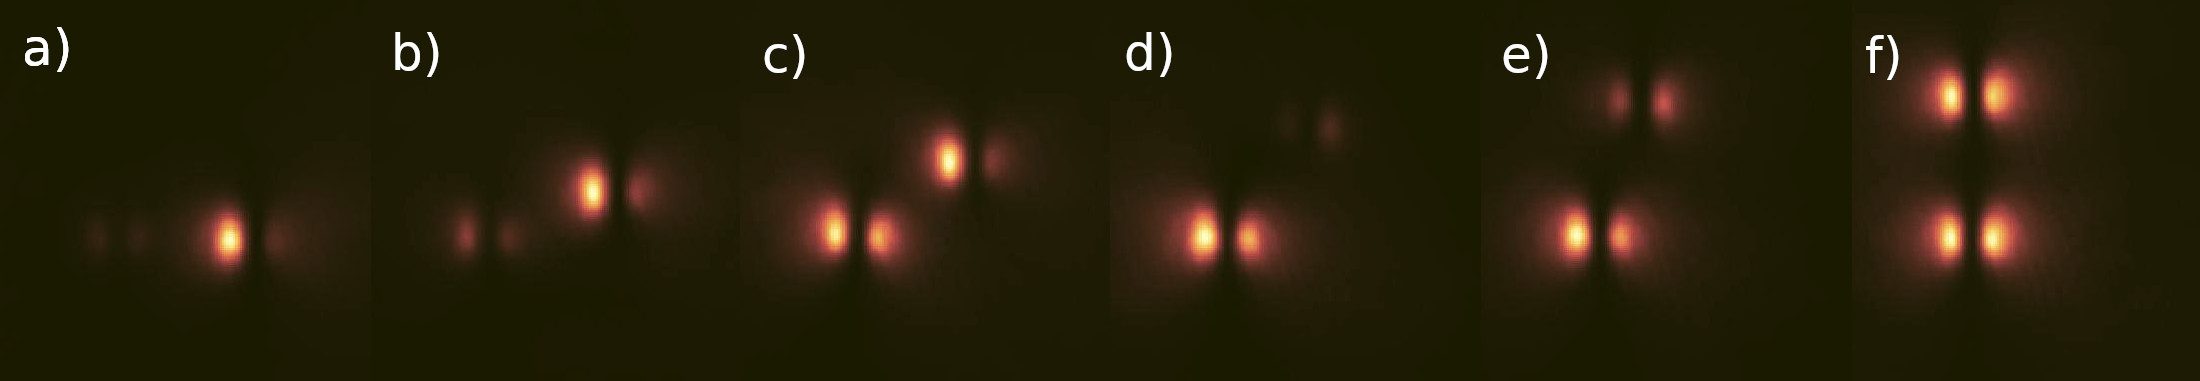
\includegraphics[width=0.9\linewidth]{./media/dipoles.jpg}
	\caption{a)-f) Barrido en ángulo de dímeros dipolares a una distancia de separación de 25 $\mu$m propagando en una distancia de 25 mm en la dirección perpendicular al plano. La inyección se realiza en la molécula inferior izquierda con un holograma tipo Hermite-Gauss TEM$_{10}$. \label{fig:dipoles}}
\end{figure}

Actualmente, se está trabajando en la excitación de un OAM con $\ell = \pm 1$ usando la técnica de modulación espacial de la Figura \ref{fig:SLM}. Los resultados iniciales muestran que la excitación de vórtices requiere una elipticidad nula con un margen de error muy pequeño. En la Figura \ref{fig:vortex}a) se demuestra la propagación de un modo Laguerre-Gauss con $\ell = +1$ a lo largo de una molécula fotónica de 9 sitios, distribuidos en forma de círculo. Para asegurar que la estructura de fase del OAM se mantiene, es necesario realizar un interferograma (ver Figura \ref{fig:vortex}b)) Se espera controlar la fabricación y excitación de guías vorticiales que nos permitan estudiar a continuación la inducción de flujos magnéticos no triviales en redes fotónicas.

\begin{figure}[H]
	\centering
	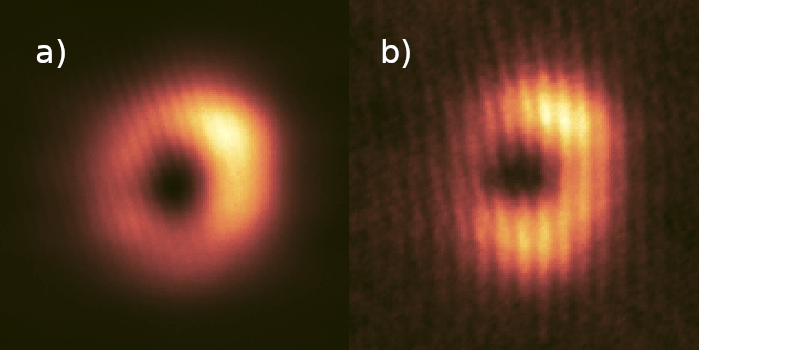
\includegraphics[width=0.5\linewidth]{./media/vortex.png}
	\caption{a) Intensidad de un OAM propagado en una molécula fotónica con $\ell = +1$. b) Interferograma que captura el cambio de fase esperado. \label{fig:vortex}}
\end{figure} 

\section{Plan de trabajo o carta Gantt}

Para la realización del trabajo de tesis se propone el siguiente plan de trabajo:

\begin{enumerate}
	\item Estimación de parámetros del perfil de índice de refracción a partir de la excitación de dímeros homogéneos y comparación con simulaciones numéricas. Mes 1.
	\item Fabricación y medición de dímeros SP y PP para caracterizar acoplamientos multiorbitales. Meses 2-3.
	\item Estudio y simulación de las redes 1D-SP y SP-SSH con particular énfasis en la naturaleza de los estados de borde y si su origen es o no topológico. Meses 4-5
	\item Simulación de redes con vórtices con efectos experimentales apreciables al cambiar el valor de la circulación $\ell$. Meses 6-7.
	\item Fabricación y medición de redes fotónicas con flujo no trivial mediante SLM y excitación por supercontinuo. Meses 7-8.
	\item Escritura y defensa de Tesis. Meses 9-12.
\end{enumerate}


% citations
\renewcommand\refname{Referencias}
\bibliographystyle{unsrtnat}


\bibliography{citations}

\end{document}
